\documentclass{beamer}

\mode<presentation> {

\usetheme{Montpellier}
}

\usepackage{graphicx} % Allows including images
\usepackage[frenchb]{babel}
\usepackage[T1]{fontenc}
\usepackage[utf8]{inputenc}
% \usepackage[demo]{graphicx}
% \usepackage{caption}

\usepackage{subcaption}
% \usepackage{subfig}
% \usepackage{algorithm,algorithmic}
\usepackage{algorithm2e}
\usepackage{listings}
% \usepackage{ntheorem}
\usepackage{booktabs} % Allows the use of \toprule, \midrule and \bottomrule in tables
\setcounter{tocdepth}{2}
\graphicspath{{../../Figures/}}

%----------------------------------------------------------------------------------------
%	TITLE PAGE
%----------------------------------------------------------------------------------------

\setbeamertemplate{title page}{
    \centering

    \Large\bfseries
    Machine Learning Tek 5: overview
    

\begin{figure}[!h]
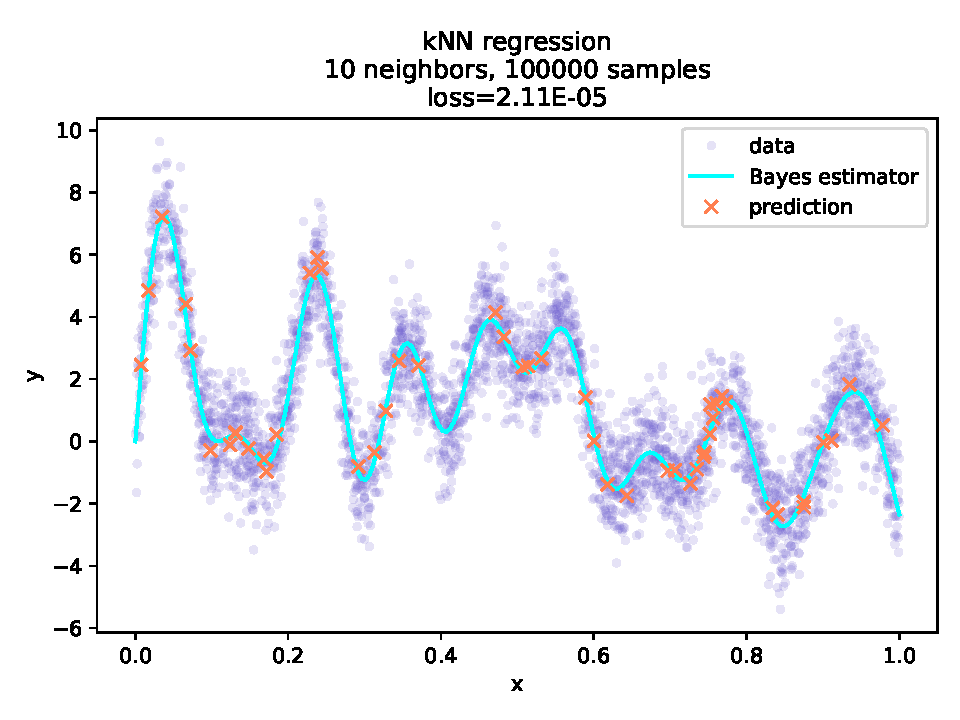
\includegraphics[width=8cm]{knn}
\end{figure}

    }

\title[FTML]{title}


\date{} % Date, can be changed to a custom date

\makeatletter
\let\@@magyar@captionfix\relax
\makeatother
\begin{document}


\frame{\titlepage}

\begin{frame}{Course repository}
	  \url{https://github.com/nlehir/ML_tek5}:
	    \begin{itemize}
		\item slides
		\item code and exercises
		\item project description
		\item other documents
		\item broad content summary (might slightly evolve) in the README.md
	    \end{itemize}
\end{frame}

\begin{frame}
\frametitle{Organization}
\begin{itemize}
	\item Presentations / discussions
	\item Coding exercises / paper+pen exercises
	\item Project: explained this afternoon
	\item \textbf{questions:} please feel free to ask questions:
	    \begin{itemize}
	    	\item you can ask directly
		\item or write them in the chat
	    \end{itemize}
	    more questions = more interesting / fun course !
\end{itemize}
\end{frame}

\begin{frame}{Practical aspects}
	\begin{itemize}
	    \item Python 3 \url{https://www.python.org/}, e.g. 3.13.2
	    \item Third-party libraries: see \textbf{requirements.txt}
	    \item Installation options are discussed in the README.md
	\end{itemize}
\end{frame}

\begin{frame}{Organization}
   \begin{itemize}
       \item \textbf{{jupyter notebooks}} are convenient python interpreters. Depending on your preference, you may use them or mere python scripts (I tend to prefer scripts but by copying and pasting, you are able to turn a script into a notebook and vice versa)
           \begin{figure}[htpb]
               \centering
               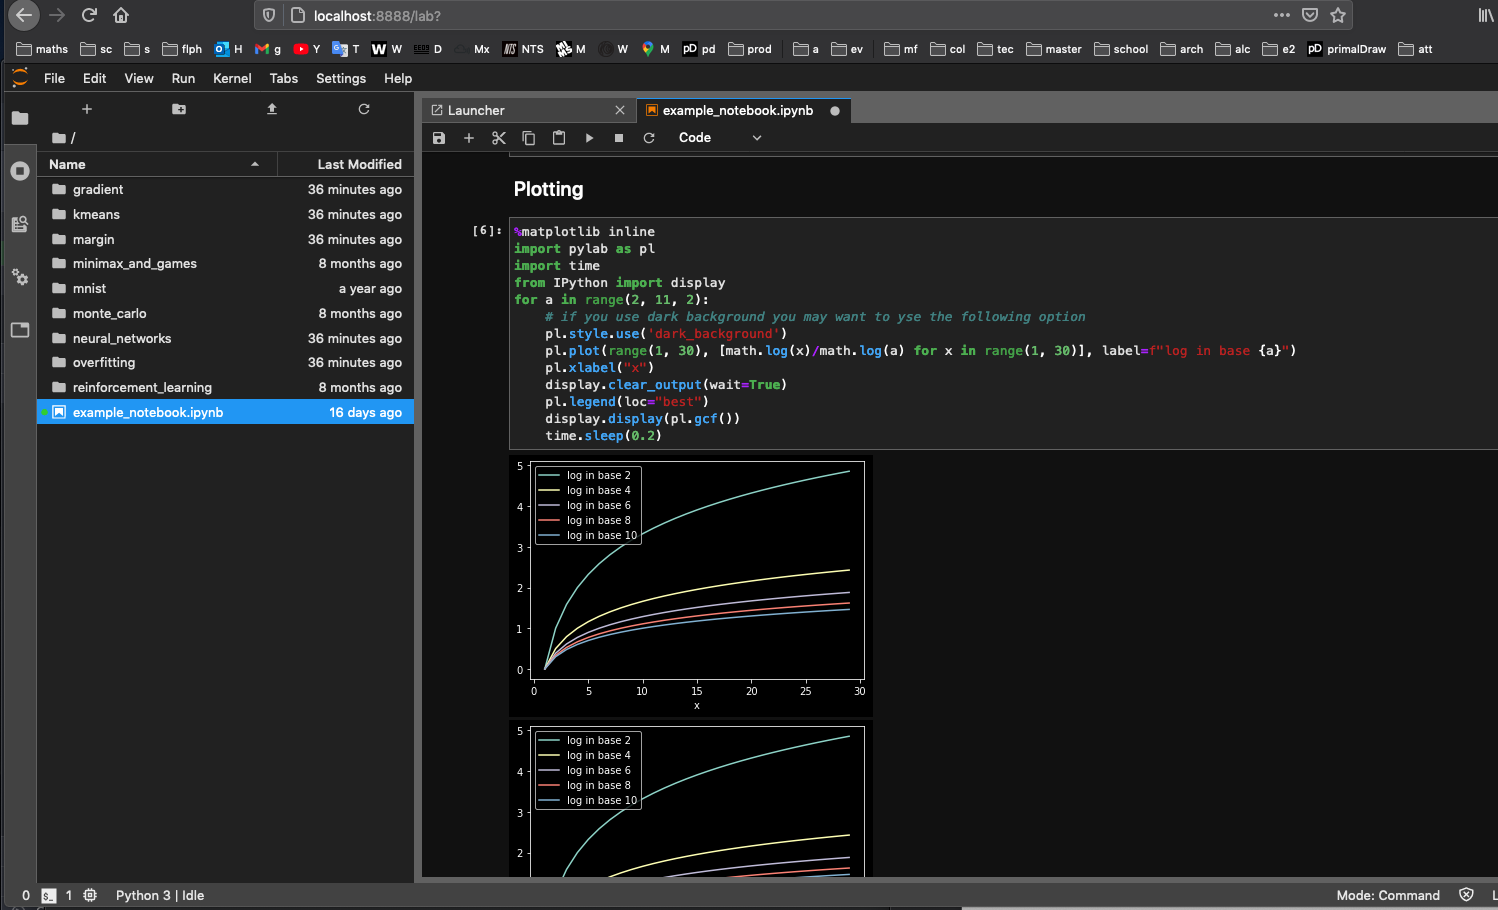
\includegraphics[width=0.6\linewidth]{notebook}
           \end{figure}
   \end{itemize} 
\end{frame}

\end{document} 
